\section{Zielsetzung}
Ziel dieses Versuchs ist es ultrakurze Laserpulse mittels der Autokorrelationsmethode zu vermessen.
Außerdem soll das Impulsdauer-Bandbreite-Produkt in Abhängigkeit von Bandpassfiltern und
der Dispersion, die der Impuls erfährt, untersucht werden.
\section{Theorie}
\subsection{Erzeugung ultrakurzer Lichtpulse}
Bei einem Dauerstrichlaser oszillieren alle Resonatormoden im Resonator ohne 
feste Phasenbeziehung. Dadurch ist das ausgekoppelte elektrische Feld zeitlich statistisch verteilt.
Um ultrakurze Lichtpulse zu erzeugen, müssen diese Moden phasengekoppelt sein (Modenkopplung).
Dadurch entsteht an der Stelle des Pulses konstruktive Interferenz und überall sonst destruktive Interferenz.
Der so entstandene intensive Puls läuft durch den Resonator und bei jedem Durchlauf durch den Resonator wird ein ultrakurzer Puls ausgekoppelt.
Bei Femtosekundenpulsen geschieht dieser Vorgang durch passive Modenkoppung, bei der der Puls durch intensitätsabhängige Verluste modelliert wird.

Ein Puls wird zeitlich kürzer, je mehr Moden im Resonator gekoppelt werden. Die Anzahl an Moden im Resonator wird durch die Bandbreite des Lasers bestimmt, es ist also für die Erzeugung
von ultraschnellen Pulsen von Vorteil ein aktives Medium mit möglichst großer Bandbreite zu wählen.

Für diesen Versuch wird ein modengekoppelter Erbium:Faser-Laser verwendet.
Bei einem Faserlaser dient eine Glasfaser als aktives Medium, in diesem Fall mit Erbium-Atomen dotiert.
Durch die entstehenden Elektron-Phonon-Wechselwirkungen verbreitern sich die Energieniveaus so stark, dass 
die Bandbreite ausreicht um Femtosekundenpulse (unter 100$\,$fs) zu erzeugen.

\subsection{Vermessung ultrakurzer Lichtpulse}
Zur Vermessung ultrakurzer Lichtpulse stehen herkömmliche Methoden, wie die Vermessung mittels Oszilloskop nicht zur Verfügung, da 
der Puls mit einem noch schnelleren Ereignis abgetastet werden müsste.
Bei der Methode der Autokorrelation, um die es in diesem Versuch geht, wird der Puls mit sich selbst abgetastet.
Dazu wird der Puls mittels eines Strahlteilers aufgeteilt.
Der eine Anteil läuft über eine variable Verzögerungsstrecke,
sodass bei diesem eine feste zeitliche Vergögerung relativ zum 
anderen Anteil des Pulses vorliegt. Beide Anteile werden schließlich in einem 
nichtlinearen Kristall zur Überlagerung gebracht.
Nun wird ausgenutzt, dass die Stärke der nichtlinear optischen Wechselwirkung vom Zeitüberlapp der beiden Anteile des Lichtimpulses abhängt.
Durch ein Variieren der Verzögerungsstrecke und damit der zeitlichen Verzögerung, lässt sich so der ultrakurze Lichtpuls vermessen.

Je nachdem, ob die Überlagerung kollinear oder nicht kollinear stattfindet, wird
zwischen interferometrischer und untergundfreier Intensitätsautokorrelation unterschieden.
Der erste Fall findet bei besonders kurzen Pulsen Anwendung und wird hier nicht weiter betrachtet.
Die untergundfreie Intensitätsautokorrelation hat den Vorteil, dass ein sehr hoher Dynamikbereich vermessen werden kann
und dadurch auch schwache Satelliten oder Echopulse in den Flanken des Pulses detektiert werden können.

Das Intensitätssignal ist dann die Faltung des ersten Pulses $ E (t)$ mit dem zweiten, zeitlich um $\tau$ verschobenen Puls $E ( t-\tau)$:

\begin{equation}
    I = \int_{-\infty}^{\infty}E^2(t)\cdot E^2(t-\tau)\,\symup{d}t
\end{equation}

\begin{figure}[H]
    \centering\captionsetup{format=plain}
    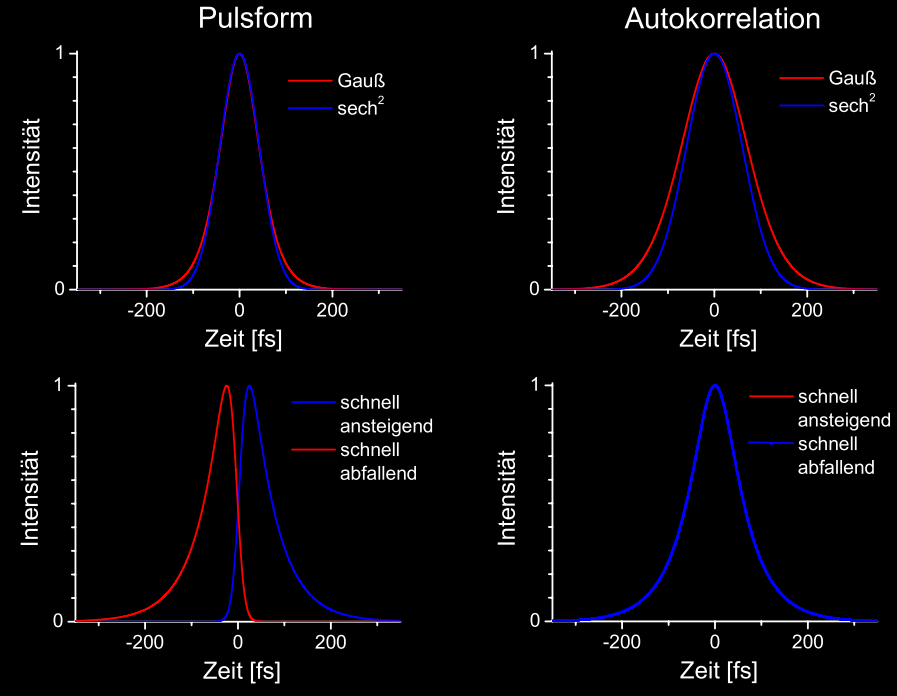
\includegraphics[width=0.9\textwidth]{bilder/AutoPulsform.png}
    \caption{Oben ist zu sehen, dass die Autokorrelation generell breiter ist als der ursprüngliche Puls. Unten ist die Problematik dargestellt, die asymmetrische Pulsformen für die Autokorrelation darstellen. Beide asymmetrischen Ausgangspulse, zeitlich gespiegelt, ergeben die gleiche Autokorrelation. Entnommen aus \cite{Pulsform}}
    \label{fig:Pulsform}
\end{figure}

Beim Vergleich der Autokorrelation mit der zugrundeliegenden Pulsform fällt genrell auf, dass die Autokorrelation breiter ist.
Dieses Verhältnis zwischen Halbwertsbreite vom ursprünglichen Puls und der Autokorrelation nennt man Entfaltungsfaktor.
Dieser liegt typischerweise zwischen 0,5 und 1. Bei einem Gaußpuls beträgt er genau $\sqrt{2}$.
Allgemein lässt sich sagen, dass sich die genaue Pulslänge nur bestimmen lässt, wenn die Pulsform bereits bekannt ist.

Alleinige Autokorrelationsmessungen geben keine vollständige Rückschlüsse auf das Pulsprofil.
So gehen beispielsweise Informationen über die Symmetrie des Pulses verloren (siehe Abbildung \ref{fig:Pulsform}).
"Frequency-ResolvedOptical Gating" (FROG) oder auch \dq Spectral Phase Interferometry for Direct ElectricField Reconstruction“ (SPIDER)
sind Methoden mit der Möglichkeit diese Nachteile zu umgehen, jedoch sind diese auch aufwändiger als die Autokorrelation.

\subsection{Summenfrequenzerzeugung}
Während bei niedrigen Laserintensitäten näherungsweise gilt, dass die Polarisation $\vec P$ linear mit dem elektrischen Feld $\vec E$ ansteigt

\begin{equation}
    \vec P = \epsilon_0 \upchi \vec E,
\end{equation}

müssen bei höheren Intensitäten auch Terme höherer Ordnung betrachtet werden:

\begin{equation}
    \vec P = \epsilon_0 (\upchi ^{(1)}\vec E+\upchi ^{(2)}\vec E^2 +...).
\end{equation}

Dabei bezeichnet $\epsilon_0$ die elektrische Feldkonstante und $\upchi ^ {(n)}$ die elektrische Suszeptibilität als Tensor n-ter Stufe.
Der nichtlineare Effekt, der sich bei der hier vorliegenden Art der Autokorrelation zunutze gemacht wird,
ist die Summenfrequenzerzeugung. Diese ist ein nicht-linearer Effekt zweiter Ordnung und kann somit nur im Materialien mit $\upchi ^ {(2)}\neq 0$ auftreten.
Zwei einfallende Photonen werden vernichtet und generieren dabei ein drittes, dessen elektrisches Feld mit der 
Summe der ursprünglichen Frequenzen schwingt. 
Es muss dabei Energie- und Impulserhaltung gelten, letztere wird später ausgenutzt um den Anteil der zweiten Harmonischen aus den Ursprungslaserstrahlen herauszufiltern.
Die Erzeugung der zweiten Harmonischen ist ein Spezialfall der Summenfrequenzerzeugung, bei der die Frequenz von zwei beitragenden Photonen gleich ist (also entsteht eine Frequenzverdopplung).



\subsection{Verlängerung der Impulsdauer}
Wie zu Beginn erwähnt, ist ein entscheidener Faktor für die Pulsdauer die Bandbreite des Lasers.
Je größer die Bandbreite, desto kürzer kann der Puls werden.
Bei einer spektralen Beschneidung im Nachhinein durch einen Interferenzfilter, wird
der Puls somit also zeitlich verlängert. 
Dabei wird die Pulsdauer durch die Fouriertransformation vom Frequenzraum in den Zeitraum bestimmt.


Ein Effekt, der den Puls verbreitert ohne eine bessere Energieauflösung zu erzeugen ist die Dispersion.
Allgemein bewirkt Dispersion, dass sich die unterschiedlichen Wellenlängenanteile der Welle unterschiedlich schnell ausbreiten.
Dies geschieht, weil jede Frequenzkomponente eine Phasenverschiebung beim Durchgang
durch ein dispersives Medium erfährt.
Es wird dabei zwischen normaler Dispersion (kurze Wellenlängen sind langsamer)und annormaler Dispersion (lange Wellenlängen sind langsamer) unterschieden.
Die eigentliche Mittenfrequenz des Pulses wird dabei nicht verändert, wohl aber die Form der Einhüllenden.

